\documentclass[12pt,letterpaper]{article}
\usepackage{graphicx,textcomp}
\usepackage{natbib}
\usepackage{setspace}
\usepackage{fullpage}
\usepackage{color}
\usepackage[reqno]{amsmath}
\usepackage{amsthm}
\usepackage{fancyvrb}
\usepackage{amssymb,enumerate}
\usepackage[all]{xy}
\usepackage{endnotes}
\usepackage{lscape}
\newtheorem{com}{Comment}
\usepackage{float}
\usepackage{hyperref}
\newtheorem{lem} {Lemma}
\newtheorem{prop}{Proposition}
\newtheorem{thm}{Theorem}
\newtheorem{defn}{Definition}
\newtheorem{cor}{Corollary}
\newtheorem{obs}{Observation}
\usepackage[compact]{titlesec}
\usepackage{dcolumn}
\usepackage{tikz}
\usetikzlibrary{arrows}
\usepackage{multirow}
\usepackage{xcolor}
\newcolumntype{.}{D{.}{.}{-1}}
\newcolumntype{d}[1]{D{.}{.}{#1}}
\definecolor{light-gray}{gray}{0.65}
\usepackage{url}
\usepackage{listings}
\usepackage{color}

\definecolor{codegreen}{rgb}{0,0.6,0}
\definecolor{codegray}{rgb}{0.5,0.5,0.5}
\definecolor{codepurple}{rgb}{0.58,0,0.82}
\definecolor{backcolour}{rgb}{0.95,0.95,0.92}

\lstdefinestyle{mystyle}{
	backgroundcolor=\color{backcolour},   
	commentstyle=\color{codegreen},
	keywordstyle=\color{magenta},
	numberstyle=\tiny\color{codegray},
	stringstyle=\color{codepurple},
	basicstyle=\footnotesize,
	breakatwhitespace=false,         
	breaklines=true,                 
	captionpos=b,                    
	keepspaces=true,                 
	numbers=left,                    
	numbersep=5pt,                  
	showspaces=false,                
	showstringspaces=false,
	showtabs=false,                  
	tabsize=2
}
\lstset{style=mystyle}
\newcommand{\Sref}[1]{Section~\ref{#1}}
\newtheorem{hyp}{Hypothesis}

\title{Problem Set 3}
\date{Due: November 11, 2024}
\author{Applied Stats/Quant Methods 1}


\begin{document}
	\maketitle
	\section*{Instructions}
	\begin{itemize}
		\item Please show your work! You may lose points by simply writing in the answer. If the problem requires you to execute commands in \texttt{R}, please include the code you used to get your answers. Please also include the \texttt{.R} file that contains your code. If you are not sure if work needs to be shown for a particular problem, please ask.
	\item Your homework should be submitted electronically on GitHub.
	\item This problem set is due before 23:59 on Sunday November 11, 2024. No late assignments will be accepted.

	\end{itemize}

		\vspace{.25cm}
	
\noindent In this problem set, you will run several regressions and create an add variable plot (see the lecture slides) in \texttt{R} using the \texttt{incumbents\_subset.csv} dataset. Include all of your code.

	\vspace{.5cm}
\section*{Question 1}
\vspace{.25cm}
\noindent We are interested in knowing how the difference in campaign spending between incumbent and challenger affects the incumbent's vote share. 
\newpage
	\begin{enumerate}
		\item Run a regression where the outcome variable is \texttt{voteshare} and the explanatory variable is \texttt{difflog}.	
			\begin{table}[!htbp] \centering 
			\caption{} 
			\label{} 
			\begin{tabular}{@{\extracolsep{5pt}}lc} 
				\\[-1.8ex]\hline 
				\hline \\[-1.8ex] 
				& \multicolumn{1}{c}{\textit{Outcome variable:}} \\ 
				\cline{2-2} 
				\\[-1.8ex] & voteshare \\ 
				\hline \\[-1.8ex] 
				difflog & 0.042$^{***}$ \\ 
				& (0.001) \\ 
				& \\ 
				Constant & 0.579$^{***}$ \\ 
				& (0.002) \\ 
				& \\ 
				\hline \\[-1.8ex] 
				Observations & 3,193 \\ 
				R$^{2}$ & 0.367 \\ 
				Adjusted R$^{2}$ & 0.367 \\ 
				Residual Std. Error & 0.079 (df = 3191) \\ 
				F Statistic & 1,852.791$^{***}$ (df = 1; 3191) \\ 
				\hline 
				\hline \\[-1.8ex] 
				\textit{Note:}  & \multicolumn{1}{r}{$^{*}$p$<$0.1; $^{**}$p$<$0.05; $^{***}$p$<$0.01} \\ 
			\end{tabular} 
		\end{table} 
		
			\lstinputlisting[language=R, firstline=1, lastline=25]{PS3.R} 
		
		
			\item Make a scatterplot of the two variables and add the regression line. 		
		\begin{figure}[H]
			\centering
			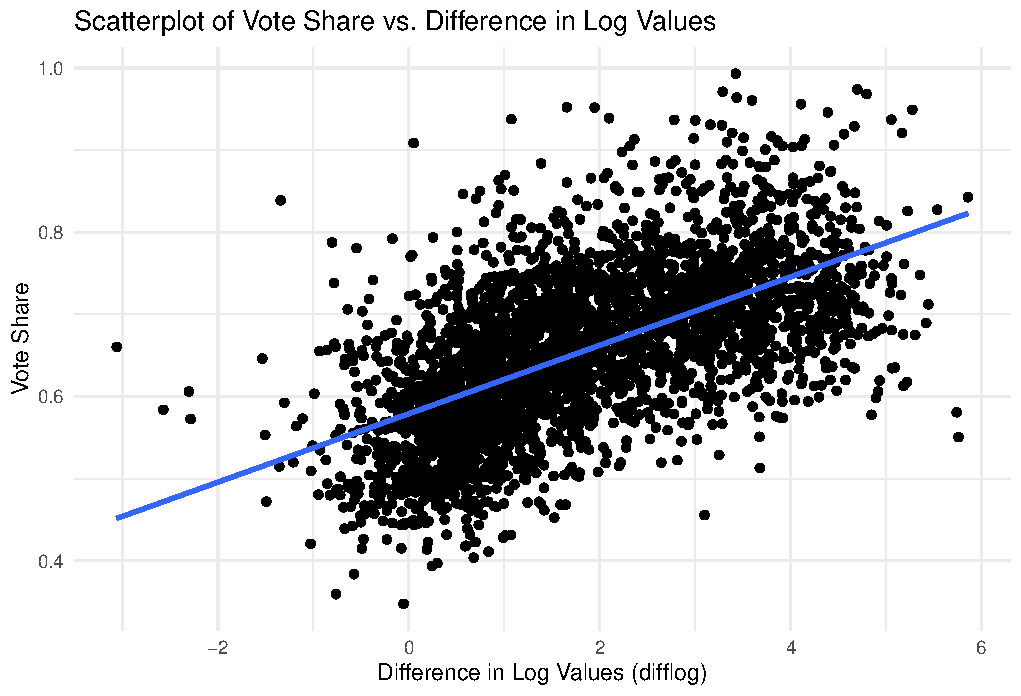
\includegraphics[width=0.7\textwidth]{ScatterPlot1.pdf}  % Adjusted to 80% of the text width
			\caption{Scatterplot of Vote Share vs Difference in Log Values}
			\label{fig:pdf}
		\end{figure}
					\lstinputlisting[language=R, firstline=27, lastline=38]{PS3.R} 
		
		\newpage
		\item Save the residuals of the model in a separate object.	
		\begin{figure}[H]
		\centering
		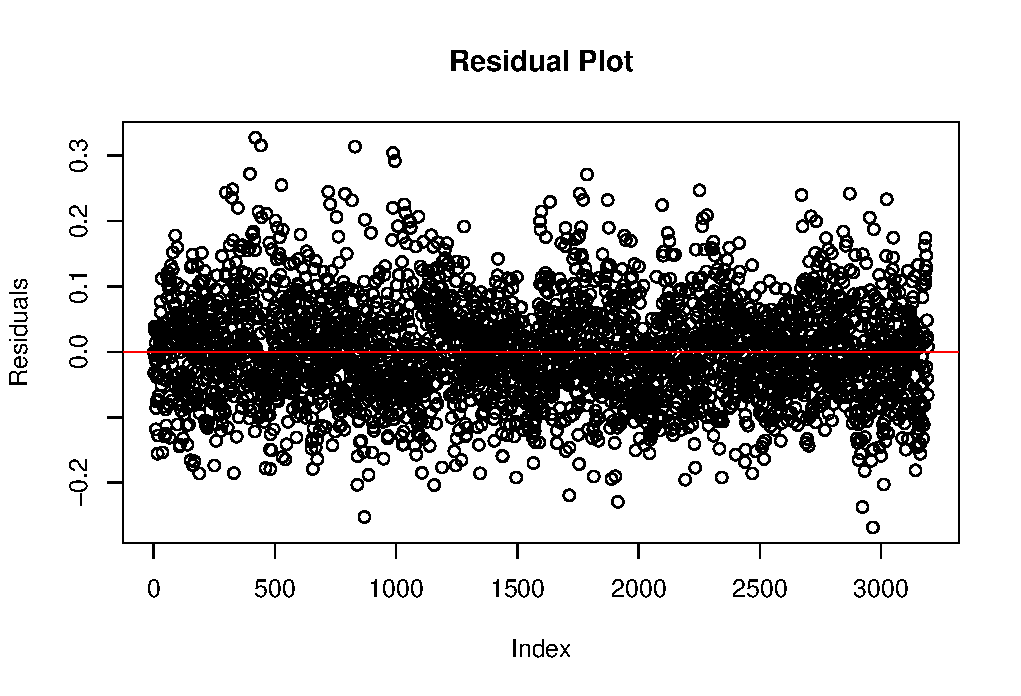
\includegraphics[width=0.7\textwidth]{ResidualPlot.pdf}  % Adjusted to 80% of the text width
		\caption{Residual Plot Visualisation}
		\label{fig:pdf}
	\end{figure}
							\lstinputlisting[language=R, firstline=42, lastline=48]{PS3.R} 
		
		\item Write the prediction equation.
	\end{enumerate}
The standard bivariate regression equation is: 

\begin{center}
	$y = \beta_0 + \beta_1 x + \epsilon$
\end{center}
For this fitted model, the dependent variable ($y$) is \texttt{voteshare}, and the independent variable ($x$) is \texttt{difflog}. The estimated intercept ($\beta_0$) is 0.579, and the estimated slope coefficient ($\beta_1$) is 0.042. Thus, the fitted model prediction equation is:
	
	\[
	\text{voteshare} = 0.579 + 0.042 \times \text{difflog} + \epsilon
	\]
	
\newpage

\section*{Question 2}
\noindent We are interested in knowing how the difference between incumbent and challenger's spending and the vote share of the presidential candidate of the incumbent's party are related.	\vspace{.25cm}
	\begin{enumerate}
		\item Run a regression where the outcome variable is \texttt{presvote} and the explanatory variable is \texttt{difflog}.
		\begin{table}[!htbp] \centering 
			\caption{} 
			\label{} 
			\begin{tabular}{@{\extracolsep{5pt}}lc} 
				\\[-1.8ex]\hline 
				\hline \\[-1.8ex] 
				& \multicolumn{1}{c}{\textit{Outcome variable:}} \\ 
				\cline{2-2} 
				\\[-1.8ex] & presvote \\ 
				\hline \\[-1.8ex] 
				difflog & 0.024$^{***}$ \\ 
				& (0.001) \\ 
				& \\ 
				Constant & 0.508$^{***}$ \\ 
				& (0.003) \\ 
				& \\ 
				\hline \\[-1.8ex] 
				Observations & 3,193 \\ 
				R$^{2}$ & 0.088 \\ 
				Adjusted R$^{2}$ & 0.088 \\ 
				Residual Std. Error & 0.110 (df = 3191) \\ 
				F Statistic & 307.715$^{***}$ (df = 1; 3191) \\ 
				\hline 
				\hline \\[-1.8ex] 
				\textit{Note:}  & \multicolumn{1}{r}{$^{*}$p$<$0.1; $^{**}$p$<$0.05; $^{***}$p$<$0.01} \\ 
			\end{tabular} 
		\end{table} 
									\lstinputlisting[language=R, firstline=57, lastline=73]{PS3.R} 
		\item Make a scatterplot of the two variables and add the regression line. 	
		
			\begin{figure}[H]
			\centering
			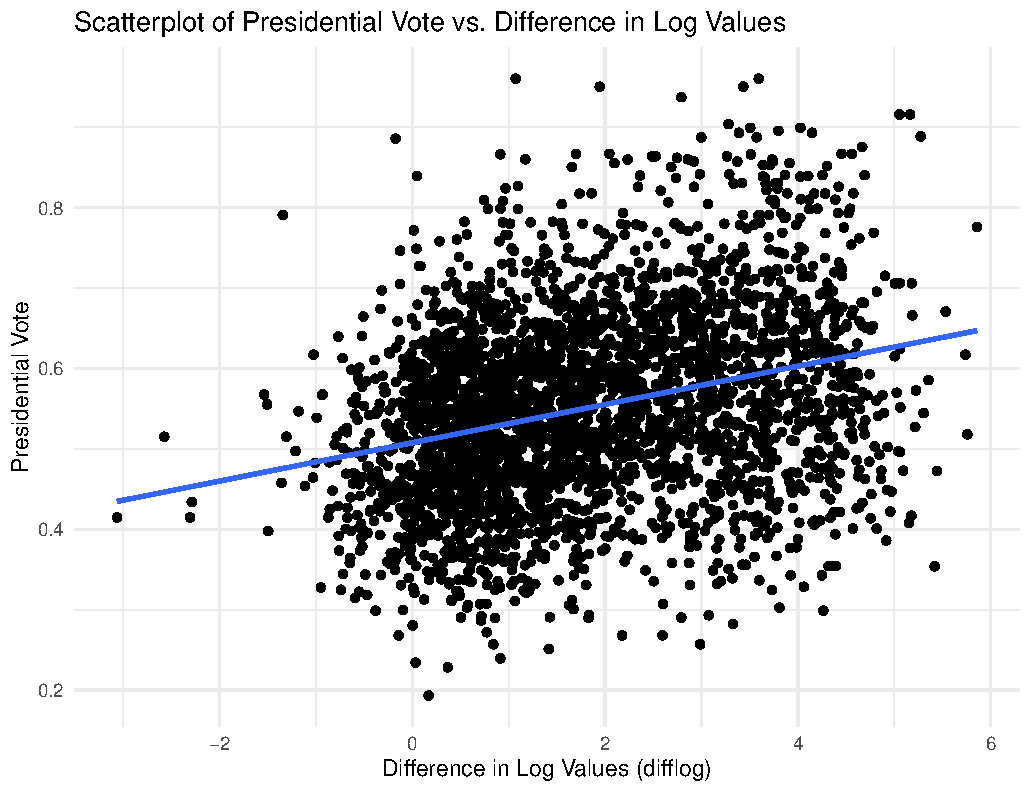
\includegraphics[width=0.7\textwidth]{ScatterPlot2.pdf}  % Adjusted to 80% of the text width
			\caption{Scatterplot of Presidential Vote vs Difference in Log Values}
			\label{fig:pdf}
		\end{figure}
											\lstinputlisting[language=R, firstline=62, lastline=74]{PS3.R} 
											\newpage
		\item Save the residuals of the model in a separate object.	\vspace{0.5cm}
			\begin{figure}[H]
			\centering
			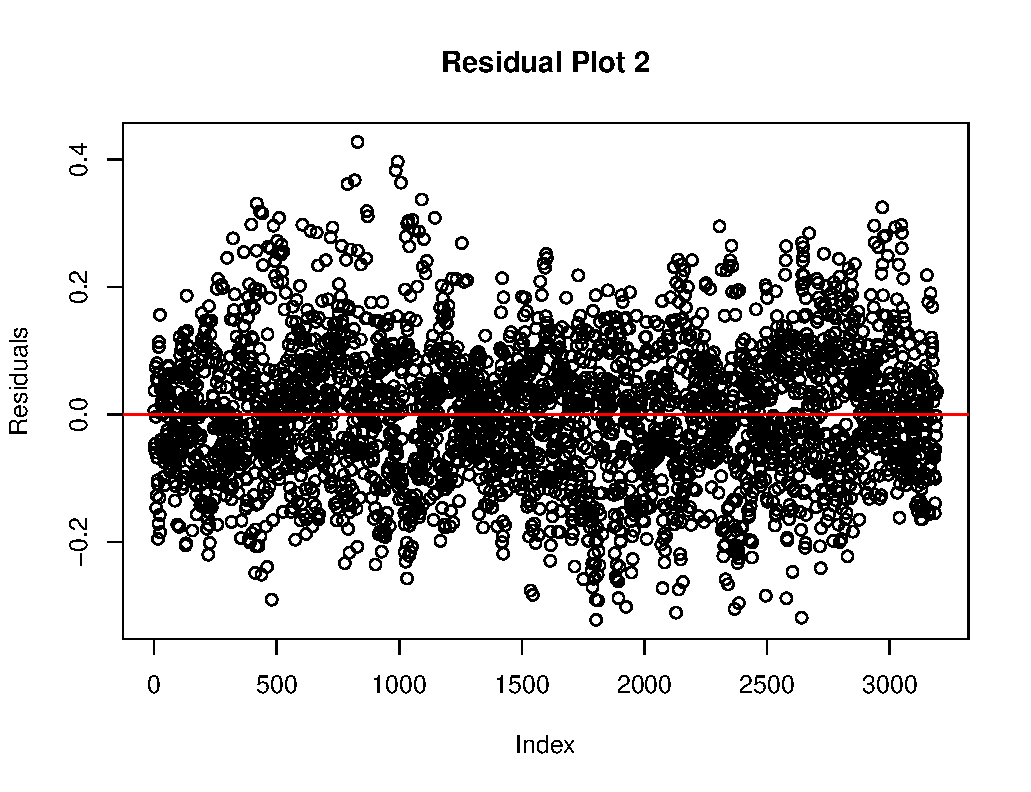
\includegraphics[width=0.7\textwidth]{ResidualPlot2.pdf}  % Adjusted to 80% of the text width
			\caption{Residual Plot Visualisation}
			\label{fig:pdf}
		\end{figure}
		
											\lstinputlisting[language=R, firstline=74, lastline=80]{PS3.R} 
		\item Write the prediction equation.
		
		The prediction equation for this model is:
		
		\[
		\text{presvote} = 0.507583 + 0.023837 \times \text{difflog} + \epsilon
		\]
		
	
		
	\end{enumerate}
	
	\newpage	
\section*{Question 3}

\noindent We are interested in knowing how the vote share of the presidential candidate of the incumbent's party is associated with the incumbent's electoral success.
	\vspace{.25cm}
	\begin{enumerate}
		\item Run a regression where the outcome variable is \texttt{voteshare} and the explanatory variable is \texttt{presvote}.
		\begin{table}[!htbp] \centering 
			\caption{} 
			\label{} 
			\begin{tabular}{@{\extracolsep{5pt}}lc} 
				\\[-1.8ex]\hline 
				\hline \\[-1.8ex] 
				& \multicolumn{1}{c}{\textit{Outcome variable:}} \\ 
				\cline{2-2} 
				\\[-1.8ex] & voteshare \\ 
				\hline \\[-1.8ex] 
				presvote & 0.388$^{***}$ \\ 
				& (0.013) \\ 
				& \\ 
				Constant & 0.441$^{***}$ \\ 
				& (0.008) \\ 
				& \\ 
				\hline \\[-1.8ex] 
				Observations & 3,193 \\ 
				R$^{2}$ & 0.206 \\ 
				Adjusted R$^{2}$ & 0.206 \\ 
				Residual Std. Error & 0.088 (df = 3191) \\ 
				F Statistic & 826.950$^{***}$ (df = 1; 3191) \\ 
				\hline 
				\hline \\[-1.8ex] 
				\textit{Note:}  & \multicolumn{1}{r}{$^{*}$p$<$0.1; $^{**}$p$<$0.05; $^{***}$p$<$0.01} \\ 
			\end{tabular} 
		\end{table} 
													\lstinputlisting[language=R, firstline=83, lastline=89]{PS3.R} 
		\newpage
		\item Make a scatterplot of the two variables and add the regression line. 
		\begin{figure}[H]
	\centering
	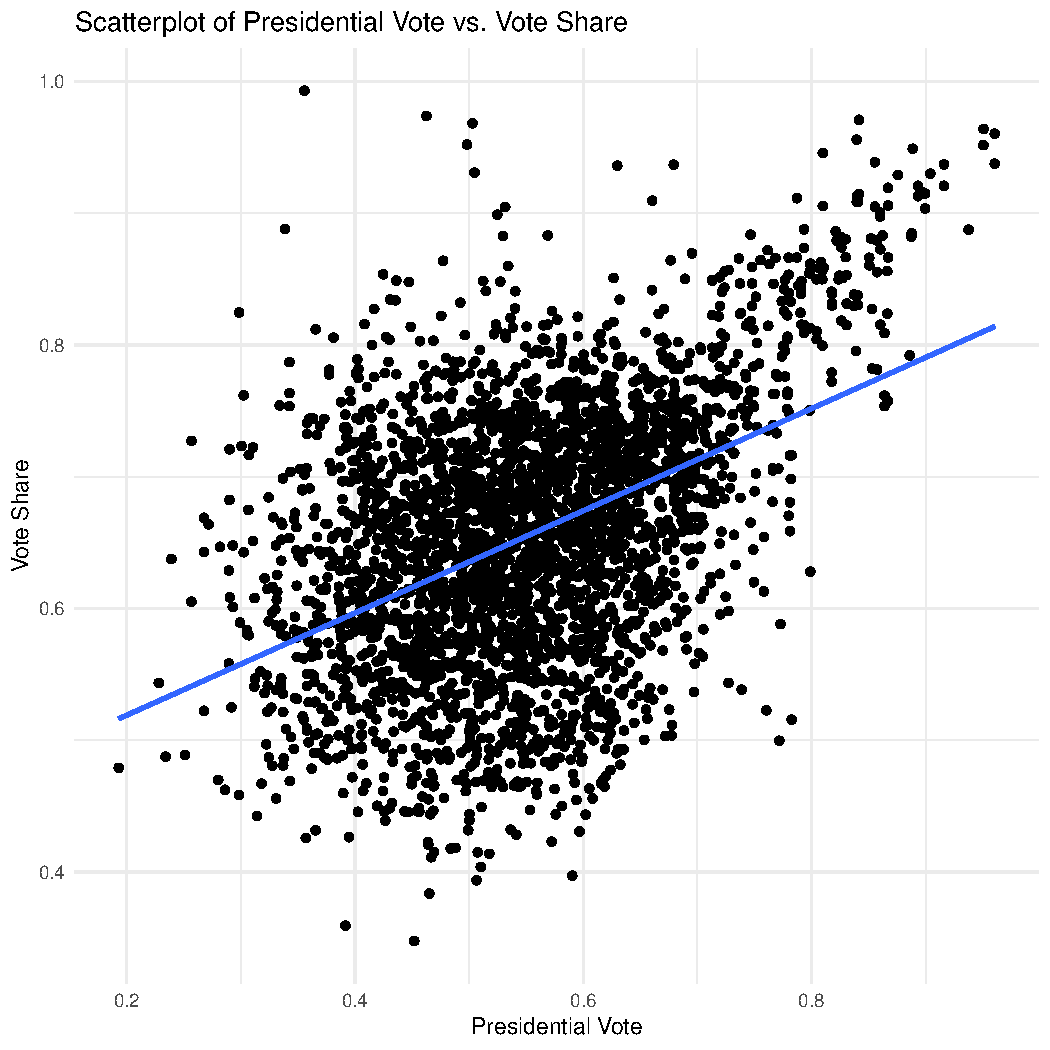
\includegraphics[width=0.7\textwidth]{ScatterPlot3.pdf}  % Adjusted to 70% of the text width
	\caption{Scatterplot of Vote Share vs Presidential Votes}
	\label{fig:pdf}
\end{figure}
											\lstinputlisting[language=R, firstline=90, lastline=101]{PS3.R} 
		\item Write the prediction equation.
		
		The prediction equation is as follows: 
\[
\text{voteshare} = 0.441330 + 0.388018 \times \text{presvote} + \epsilon
\]

	\end{enumerate}


\newpage	
\section*{Question 4}
\noindent The residuals from part (a) tell us how much of the variation in \texttt{voteshare} is $not$ explained by the difference in spending between incumbent and challenger. The residuals in part (b) tell us how much of the variation in \texttt{presvote} is $not$ explained by the difference in spending between incumbent and challenger in the district.
	\begin{enumerate}
		\item Run a regression where the outcome variable is the residuals from Question 1 and the explanatory variable is the residuals from Question 2.	
\begin{table}[!htbp] \centering 
	\caption{} 
	\label{} 
	\begin{tabular}{@{\extracolsep{5pt}}lc} 
		\\[-1.8ex]\hline 
		\hline \\[-1.8ex] 
		& \multicolumn{1}{c}{\textit{Dependent variable:}} \\ 
		\cline{2-2} 
		\\[-1.8ex] & residuals\_object \\ 
		\hline \\[-1.8ex] 
		residuals\_object2 & 0.257$^{***}$ \\ 
		& (0.012) \\ 
		& \\ 
		Constant & $-$0.000 \\ 
		& (0.001) \\ 
		& \\ 
		\hline \\[-1.8ex] 
		Observations & 3,193 \\ 
		R$^{2}$ & 0.130 \\ 
		Adjusted R$^{2}$ & 0.130 \\ 
		Residual Std. Error & 0.073 (df = 3191) \\ 
		F Statistic & 476.975$^{***}$ (df = 1; 3191) \\ 
		\hline 
		\hline \\[-1.8ex] 
		\textit{Note:}  & \multicolumn{1}{r}{$^{*}$p$<$0.1; $^{**}$p$<$0.05; $^{***}$p$<$0.01} \\ 
	\end{tabular} 
\end{table}
		
													\lstinputlisting[language=R, firstline=105, lastline=112]{PS3.R} 
													\newpage
		\item Make a scatterplot of the two residuals and add the regression line. 
			\begin{figure}[H]
			\centering
			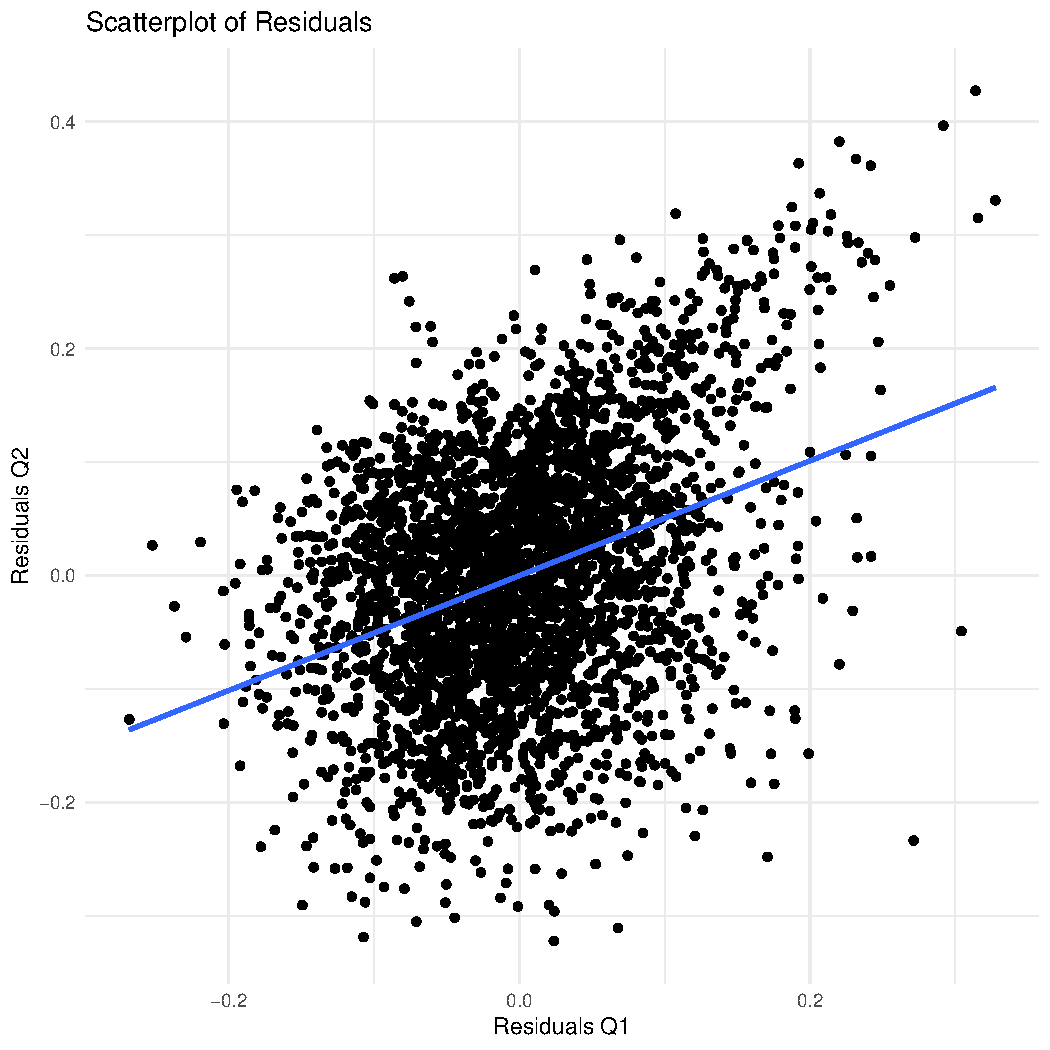
\includegraphics[width=0.7\textwidth]{ScatterPlot4.pdf}  % Adjusted to 70% of the text width
			\caption{Scatterplot of Residuals}
			\label{fig:pdf}
				\lstinputlisting[language=R, firstline=114, lastline=125]{PS3.R} 
		\end{figure}
		\item Write the prediction equation.
\[
\text{residuals\_object} = -1.942 \times 10^{-18} + 0.2569 \times \text{residuals\_object2} + \epsilon
\]
	
		
	\end{enumerate}
	
	\newpage	

\section*{Question 5}
\noindent What if the incumbent's vote share is affected by both the president's popularity and the difference in spending between incumbent and challenger? 
	\begin{enumerate}
		\item Run a regression where the outcome variable is the incumbent's \texttt{voteshare} and the explanatory variables are \texttt{difflog} and \texttt{presvote}.	
		\begin{table}[!htbp] \centering 
			\caption{} 
			\label{} 
			\begin{tabular}{@{\extracolsep{5pt}}lc} 
				\\[-1.8ex]\hline 
				\hline \\[-1.8ex] 
				& \multicolumn{1}{c}{\textit{Dependent variable:}} \\ 
				\cline{2-2} 
				\\[-1.8ex] & voteshare \\ 
				\hline \\[-1.8ex] 
				difflog & 0.036$^{***}$ \\ 
				& (0.001) \\ 
				& \\ 
				presvote & 0.257$^{***}$ \\ 
				& (0.012) \\ 
				& \\ 
				Constant & 0.449$^{***}$ \\ 
				& (0.006) \\ 
				& \\ 
				\hline \\[-1.8ex] 
				Observations & 3,193 \\ 
				R$^{2}$ & 0.450 \\ 
				Adjusted R$^{2}$ & 0.449 \\ 
				Residual Std. Error & 0.073 (df = 3190) \\ 
				F Statistic & 1,302.947$^{***}$ (df = 2; 3190) \\ 
				\hline 
				\hline \\[-1.8ex] 
				\textit{Note:}  & \multicolumn{1}{r}{$^{*}$p$<$0.1; $^{**}$p$<$0.05; $^{***}$p$<$0.01} \\ 
			\end{tabular} 
		\end{table}
		\item Write the prediction equation.	
		\[
		\text{voteshare} = 0.4486442 + 0.0355431 \times \text{difflog} + 0.2568770 \times \text{presvote} + \epsilon
		\]
		
		\item What is it in this output that is identical to the output in Question 4? Why do you think this is the case?
	\end{enumerate}

The regression of the residuals in Table 4 reveals a positive and statistically significant coefficient (0.257), this coefficient is identical to the presvote coefficient in Table 5 (again, 0.257). This indicates that the unexplained variation in voteshare is positively associated with the unexplained variation in presvote. The fact that the coefficient for presvote is identical in Table 5 suggests a strong relationship between the residuals of voteshare and presvote, which is not affected when we control for differences in campaign spending

	\lstinputlisting[language=R, firstline=128, lastline=132]{PS3.R} 

\end{document}
